\section{Overview of Future Research}
Overview of major questions DNA replication , genome integrity, assembly and transcription

We are committed to rigorous and reproducible research. All experiments are performed at a minimum in biological replicate and robust statistical approaches are utilized to ensure significance.  To guarantee reproducibility of our bioinformatic approaches all of our analyses from raw data to figure are scripted and hosted on Duke's GitLab.

\sheading{DNA replication and genome integrity}
Coupling of helicase activity with the replisome and active replication is critical for maintaining genomic stability.  Uncoupling of the helicase from active DNA replication can result in the generation of ssDNA tracts which are not only susceptible to DNA damage\citep{}, but can also lead to replication catastrophe via the sequestration of RPA\citep{toledo,ercilla}.  Helicase uncoupling can be induced by a number mechanisms including limiting dNTP pools, chemical inhibition of polymerases, and by lesions (\eg bulk aducts) that block the replisome. We induced helicase uncoupling at the origin using a very tight conditional allele of Pol1/Cdc17 to prevent RNA priming by Pol alpha/primase\citep{}.  As the cells entered S-phase in the absence of DNA replication, the CMG helicase complex was activated and proceeded to unwind approximately 1 kb of DNA surrounding the origin before the holohelicase complex stalled.  

We will identify the mechanism(s) that function as a 'dead man's switch' to limit helicase progression in the absence of DNA replication.  Helicase progression may be limited by sequence, topological constraints, limiting RPA, or Rad53-mediated phosphorylation.  We found that the CMG helicase complex stalled in regions of elevated GC content relative to the origins of DNA replication.  We will explicitly test the role of sequence features in limiting helicase movement by inserting synthetic sequences of approximately 1 kb with differing GC-content adjacent to an early efficient origin.  Alternatively, topological constraints may limit helicase progression in the absence of active DNA replication. We will manipulate the levels of yeast topoisomerases top1 and top2 by chemical inhibition, knockout and overexpression and assess helicase progression.   Rad53 has been linked helicase speed and progression both directly and indirectly via regulation of dNTP levels.  At the population level, we did not observe a difference in helicase progression in the absence of mrc1 or activated rad53; however, we only examined the distribution of the helicase at 40 minutes post alpha factor release and later time points. We will examine earlier timepoints and also hope to take advantage of long read single molecule sequencing to precisely map where the helicase stalls on indvidual DNA fragments as the population data may be obscuring finer grained control of rad53-mediated helicase progression.



% Failure to regulate helicase uncoupling at the origin via a “dead man's switch” may trigger replication catastrophe resulting from the generation of excess ssDNA and the sequestration of RPA (Toledo et al. 2013; Ercilla et al. 2020); 

%Mcm dead man switch -- what's regulating GC, topological, extrinsic signalling.

A core tenet of the cell cycle is that the entire genome must be duplicated once and only once during S-phase.  The distribution and ordered activation of replication origins, the bi-directional nature of DNA replication, and cell cycle checkpoints all ensure that the genome is completely copied prior to entering mitosis. Failure to completely copy the genome may result in a catastrophic failure to segregate the chromosomes and potentially result in chromotripsis.   

A consequence of the CMG-helicase complexes stalling on either side of the origin is that upon restoration of priming activity, the helicases will be oriented to unwind DNA away from the origin, potentially leaving a stretch of unreplicated duplex DNA at the origin.  Consistent with this hypothesis, cells with restored priming experienced a prolonged delay in G2/M due to the presence of unreplicated DNA at the origin\citep{}.  However, this delay is transient and the cells are eventually able to recover and resume normal cell cycling, suggesting that mechanism(s) must exist to deal with short un-replicated gaps.

We will identify the mechanism(s) by which the cells are able to resolve un-replicated gaps in their chromosomes.  We hypothesize that alternative helicases will be recruited to the unreplicated duplex DNA to facilitate unwinding and synthesis.  We will start with a target genetic screen of non-replicative helicases (pif1, rrm3, sgs, srs1, mpgh, dna2) involved in DNA repair and maintenance.  We will analyze the ability of cells (eg. cdc17ts pif1) to recover from the transient loss of priming.  Our preliminary data indicate that cells with short unreplicated gaps at origin sequences require Pif1 for viability and that in the absence of Pif1 they accumulate in early anaphase with a failure to segregate their genomes.  We will continue to screen additional helicases as there will likely be multiple factors involvedin resolving these structures.  We will use live imaging (LoS Danny Lew, Duke) to quantify the delay in progression through mitosis for each of the mutant strains.  Finally, it is worth noting that the intermediate we have identified (short un-replicated stretches of DNA) are structurally similar to intermediates predicted to occur from defects in the termination of DNA replication. Similar to the elegant \invitro work from the Labib group, we also find that the helicase pif1 is required for resolving these structures and progressing through anaphase.  Something about this being a model for termination studies. 
\begin{floatingfigure}[lt]{3.8in}
\vspace{-4mm}
\begin{center}
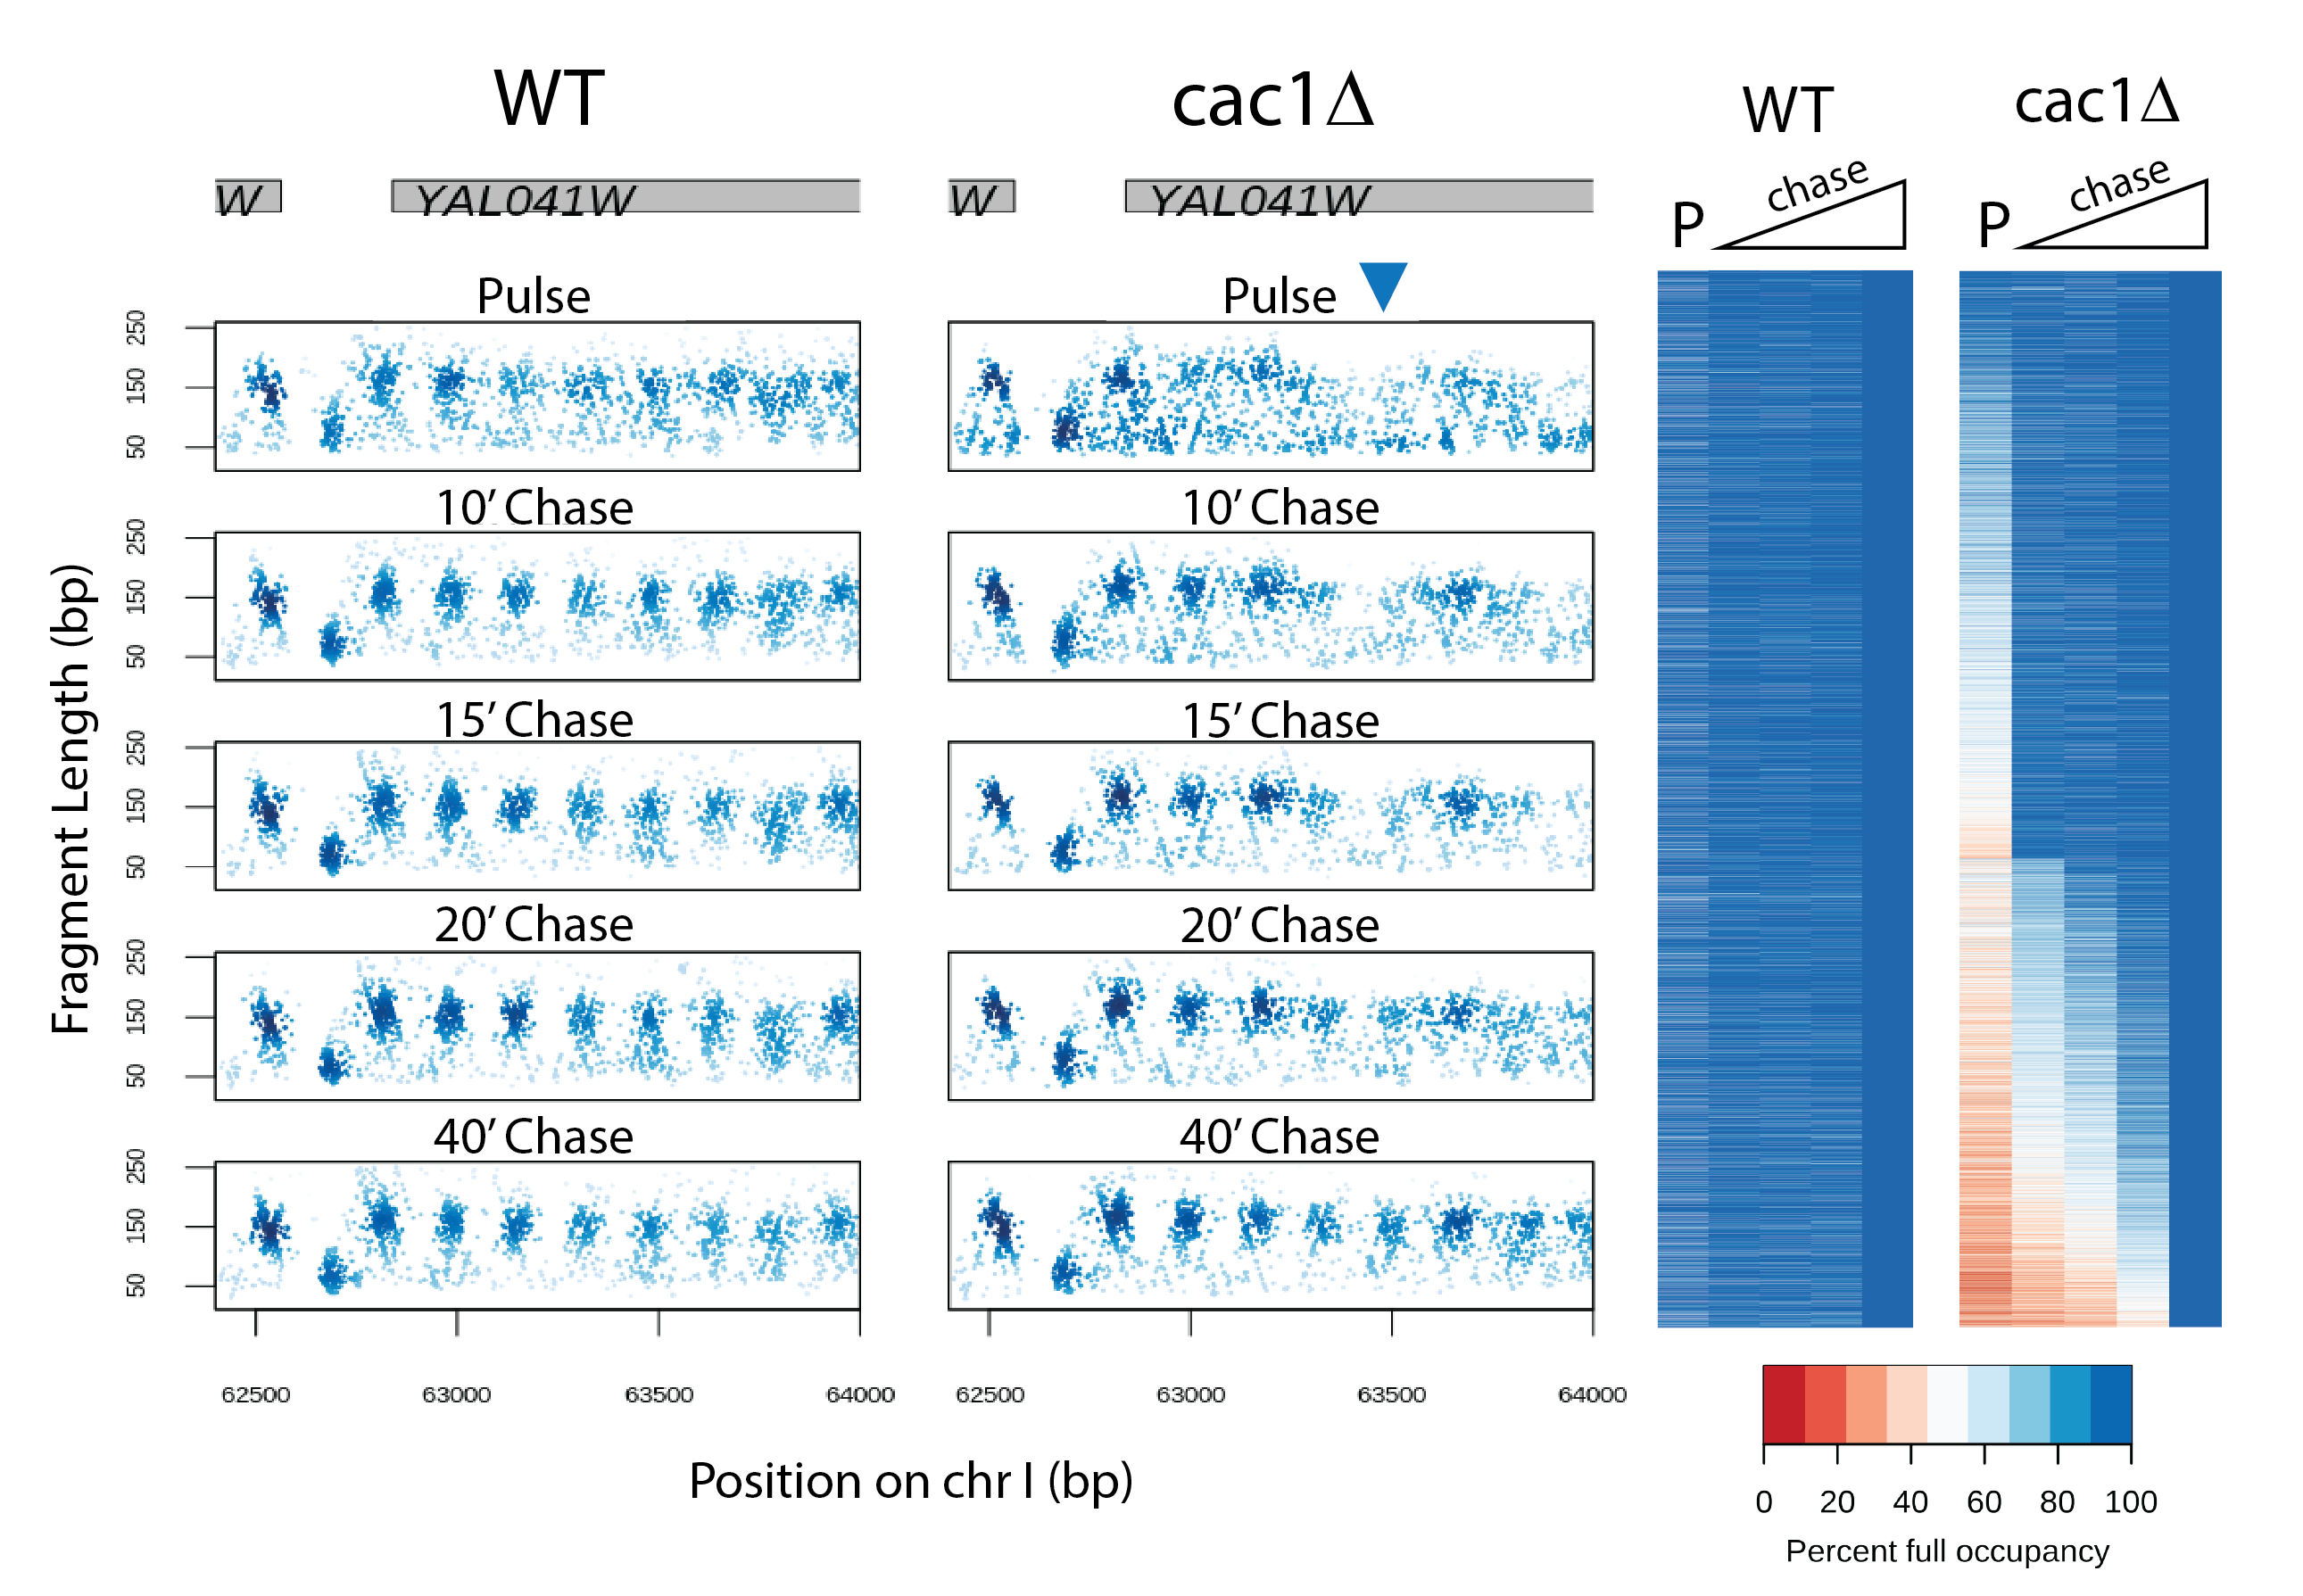
\includegraphics[width=3.8in]{r35_figures/cac_typhoon_heatmap_dm.png}
\end{center}
\vspace{3mm}
\caption{Nascent GCOPs reveal heterogeneous nucleosome deposition in \cac cells.  MNase protected DNA fragments were subjected to paired-end sequencing and the resulting fragment lengths were plotted as a function of chromosomal position.  Well phased fragments at $\sim$150 bp represent sequences protected by nucleosomes (red ovals in cartoon) and smaller fragments represent other DNA binding factors (\eg ORC at the ACS and Abf1).  In an \textit{ORC1-161} mutant the footprint at the ACS disappears at the non-permissive temperature.}%
\end{floatingfigure}%

\sheading{Chromatin assembly behind the fork}
Passage of the DNA replication fork through chromatin results in the transient disassembly of nucleosomes at the fork and their re-assembly on the two nascent daughter strands behind the fork.  Chromatin assembly on nascent DNA is a complex and regulated process that is critical for preserving epigenetic information.  A major question is understanding how specific histone chaperones contribute to and facilitate the spatiotemporal kinetics of nucleosome deposition and chromatin assembly behind the replication fork. 


% DNA replication results in the complete disassembly of chromatin, which must be re-established behind the replication fork in order to propagate the original epigenetic state. Chromatin restoration on nascent DNA is a complex and regulated process, including nucleosome assembly, remodeling, and deposition of histone variants\citep{MacAlpine2013-ds}.



% Introduction paragraph on the inheritance of epigenetic state including parental and nascent histones -- development, unidirectional inheritance.

 In preliminary experiments, we have focused on the role of the Caf-1 complex which is involved in the replication-dependent deposition of nascent histone H3-H4 tetramers during S-phase\citep{}.  In yeast cells, loss of \CAC, which encodes the largest subunit of the Caf-1 complex results in silencing defects\cite{}, increased sensitivity to DNA damage\cite{}, and elevated cryptic transription\cite{}. However, despite these phenotypes there are very little observed differences in the steady state distribution and occupancy of nucleosomes throughout the genome.  We used our nascent genome wide occupancy profiling\citep{Gutierrez2019-kw} to characterize the spatiotemporal dynamics of chromatin assembly behind the replication fork in wildtype and \cac cells (Figure 3).  We found that fully mature chromatin (45 minute chase) was nearly indistinguishable between wildtype and \cac cells.  Despite the similarities in mature chromatin we observed dramatic differences in the kinetics of chromatin maturation.  Wild type cells were able to rapidly re-establish nucleosome occupancy and organization (10 min chase); however, the chromatin of \cac cells was significantly more disorganized during the pulse and early chase periods.  Strikingly, we observed that the deposition rate of individual nucleosomes was heterogeneous, with  nucleosomes being deposited with either `fast' or `slow' kinetics.  

We hypothesize that \cac phenotypes are not due to differences in steady state chromatin architecture, but rather arise from the transient differences in chromatin assembly during S-phase.  For example, the increase in cryptic transcripts observed in \cac cells may be due to the transient exposure of cryptic promoters at the locations of `slow' nucleosome deposition during chromatin maturation.  We will explicitly test this hypothesis by using TSS-seq to capture the 5' capped end of nascent mRNAs\citep{}.  We expect to observe increased cryptic transcription initiating from the locations of `slow' nucleosomes.  We are also interested in understanding the mechanism(s) by which individual nucleosomes are deposited with heterogenous kinetics.  For example, the 'slow' nucleosomes may represent nascent histone tetramers that are deposited considerably after passage of the replication fork, or perhaps they represent histone tetramers that are deposited with the fork, but fail to incorporate two dimes of H2A/H2B to complete and stabilize the histone octamer.  We will use ChIP-exo with antibodies directed against H3K56Ac (nascent) or H3k4Me3 (mature) to precisely map the location of nascent and mature histone octamers and H3/H4 tetramers in synchronized cells following release into S-phase to distinguish among these models.  Alternatively biochemical and structural studies suggest that the Caf-1 complex forms a scaffolding structure with DNA via the K/E/R and WHD domains of Cac1 which while dispensable for \invitro deposition of H3/H4 tetramers, show defects in replication coupled nucleoasome assembly assays\citep{Sauer2018-gr, Sauer2017-es}.  We will delete the K/E/R and WHD domains of Cac1 to test the hypothesis that the DNA interaction of Cac1 may promote the deposition H3/H4 tetramers in sequences that are recalcitrant  to nucleosome formation\citep{Segal2006-tj} to ensure proper nucleosome phasing.  

The inheritance of epigenetic state behind the fork is facilitated by the local recycling and deposition of parental H3/H4 tetramers to the nascent DNA.  A number of replisome components function as histone chaperones at the fork including Mcm2, RPA and pol delta.  

In contrast to espan which provides a static read out of 



%of histone chaperones in the deposition of kinetics of nascent and parental histone across the entire genome.

%The re
% DNA replication results in the complete disassembly of chromatin, which must be re-established behind the replication fork in order to propagate the original epigenetic state. Chromatin restoration on nascent DNA is a complex and regulated process, including nucleosome assembly, remodeling, and deposition of histone variants\citep{MacAlpine2013-ds}.  Recently, proteomic techniques have been developed to study the proteins associated with replicative chromatin in a temporal fashion\citep{Alabert2014-io,Sirbu2011-wx}. %Nascent and mature chromatin are differentiated by the incorporation of nucleoside analogs (e.g. BrdU, EdU) followed by the immunoprecipitation of labeled chromatin after a short pulse of only a few minutes for nascent chromatin or followed by a longer chase period for mature chromatin. 
% While these approaches focus on studying large pools of proteins associated at multiple phases of replication, they do not provide the spatial or temporal information of chromatin maturation at individual loci. 


% caf-1 nucleosome
% other chaperones 
% provides dynamic information and strand specific
% %\sheading{DNA repair}
% %We investigated chromatin by NHEJ -- can individually lable
% local view inheritance direction
\begin{floatingfigure}[rt]{2in}%
\vspace{-4mm}%
\begin{center}%
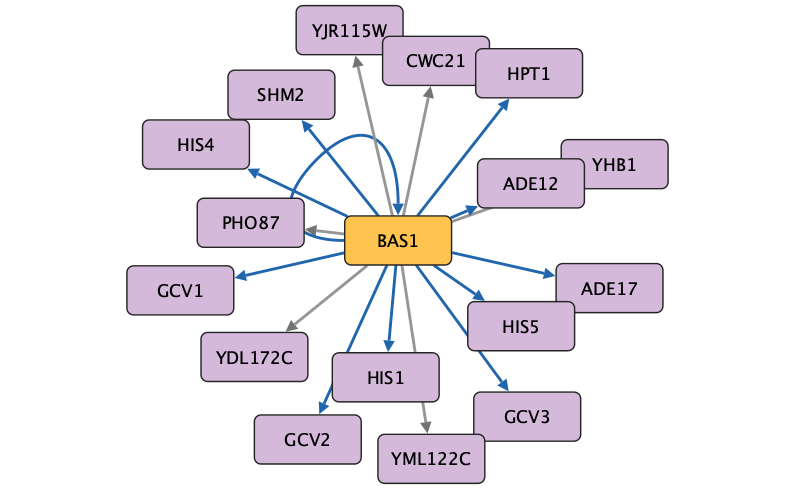
\includegraphics[width=2in]{r35_figures/BAS1_network.png}%
\end{center}%
\vspace{3mm}%
\caption{\BAS chromatin-based regulatory network.  Nodes represent genes with altered chromatin in the promoter region in bas cells.  The edges represent gene expression changes with blue being a decrease in gene expression in bac cells. Gray edges represent no detectable gene expression change despite a pronounced chromatin change in the promoter.  We are able to disambiguate direct and indirect chromatin changes by the loss of the Bas1 footprint at sites with a motif versus other chromatin changes at sites lacking a motif.}%
\end{floatingfigure}%

\sheading{Gene regulation}%
A major challenge in genome biology is deciphering the complex regulatory code embedded within the chromatin landscape to model and predict gene expression. 
Gene regulatory networks have been inferred  from the analysis of gene expression across a collection of yeast transcription factor deletion mutants\citep{Hu2007-fs,Kemmeren2014-el}.  Despite the power of these approaches, it is difficult to determine if the observed interactions are direct or indirect. Similarly, ChIP based approaches to identify the binding sites of specific TFs are prone to false positives\citep{Teytelman2013-id} and only reveal potential direct interactions for one factor at a time.  To overcome these shortcoming we generated GCOPs from 201 yeast strains harboring individual deletions of transcription regulators.  This factor agnostic approach reveals not just the loss of chromatin occupancy at \emph{bona fide} binding sites for specific factors ({\color{dukeblue}\textbf{Figure 1}}), but also reveals indirect changes in chromatin including the loss and gain of downstream regulatory factors and disrupted nucleosomes associated with active transcription.  We are able to recapitulate known gene expression networks solely from the changes in chromatin occupancy and nucleosome organization ({\color{dukeblue}\textbf{Figure 4}}).  We are also able to capture chromatin perturbations that are not associated with differential gene expression nor would they have been captured in prior gene expression based regulatory networks.  These locus specific chromatin changes independent of gene expression may serve to prime the locus for a subsequent or future transcriptional response\citep{altman}. Together with the Hartemink group at Duke (LoS Hartemink) we are now generating larger and more complex regulatory networks that integrate chromatin perturbations with gene expression.    


\sheading{Technology development}
Our GCOP assay is able to resolve regions of protected DNA occupancy at near nucleotide resolution.  We have continued to develop and extend this assay to describe the chromatin occupancy of nascent DNA as well as strand specific nascent DNA.  However, a caveat of our assay is that it is a population based assay and it is difficult to detect transient and/or rare DNA binding events.  We would like to develop a single molecule read out of chromatin occupancy that would describe the precise chromatin occupancy status for an entire single chromosome or large chromosomal fragment with binary precision.  Recent advances in next generation long read technologies (\eg Nanopore, PacBio) allow the direct read out of modified bases (eg. m6A methylation)/citep{} or nucleotide analogs (\eg BrdU)\citep{Muller2019-hd, Hennion2020-on}.  Long read sequencing coupled with the read out of m6A methylation led to the development of Fiber-seq which uses a non-specific m6A methyltransferase to methylate accessible adenine residues (Stergachis et al., 2020) as a read out of chromatin occupancy.  Historically, the very first locus specific chromatin occupancy maps were generated by the chemical treatment of chromatin with DMS (dimethyl sulfate) and the non-specific methylation of accessible purines in the DNA. More recently,  DMS-seq was developed to map chromatin accessibility following the enrichment of methylated residues by immunoprecipitation and next-generation Illumina short read sequencing (Umeyama et al., 2017).  We propose to adapt DMS-seq for use on long read sequencing platforms with direct readout of methylated purines to provide precise chromatin occupancy maps for indvidual molecules of DNA.   Alternatively, we will adapt Fiber-seq for the analysis of yeast chromatin.  Each approach presents complex analysis challenges for interpretation of the data including the sparseness of modifications in the enzyme based Fiber-seq system and deciphering the complex signal arising from potentially methylating all exposed purines with DMS.  These are not trivial challenges but our long time collaborator, Alex Hartemink, has experience developing statistical models for dealing with sparseness in single cell RNA-seq datasets\citep{} as well as developing robust sequence based models for accessibility which will help guide the interpretation of the complex DMS-seq data (LoS Hartemink).  A single molecule view of chromatin occupancy will allow us to address multiple fundamental questions in DNA replication, repair and transcription including providing a quantitative assessment of ORC, helicase loading and activation at replication origins in individual cells.

 

%Combined with chemical (DMS) or catalytic cleave (enzymatic) it should be possible to 

